
%%%%%%%%%%%%%%%%%%%%%%%%%%%%%%%%%%%%%%%%%%%%%%%%%%%%%%%%%%%%%%%%%%%%%%%%%%%%
%%%%%%%%%%%%%%%%%%%%%%%%%%%%%%%%%%%%%%%%%%%%%%%%%%%%%%%%%%%%%%%%%%%%%%%%%%%%
%%%%%%%%%%%%%%%%%%%%%%%%%%%%%%%%%%%%%%%%%%%%%%%%%%%%%%%%%%%%%%%%%%%%%%%%%%%%

\begin{frame}{Weighted Z-estimators.}

\onslide<3->{\hspace{3em}\textbf{weighted} \vspace{-0.2em}
\hspace{10em}\textbf{weighted} \vspace{-0.5em}}

We study \only<3->{ $\wedge$ }
``Z-estimators,'' i.e., roots of
\only<3->{ $\wedge$ }estimating equations.

Suppose we have $N$ data points $\d_{1}, \ldots, \d_{N}$.  Then:
%
\begin{align*}
%
\thetahat \only<4->{\color{red} (\w) \color{black}} :=
\theta \,\, \textrm{ such that } \,\,
\sumn
\only<4->{ \color{red} \w_{n} \color{black}}
G(\theta, \d_{n}) =  \zP .
%
\end{align*}
%

\onslide<2->{
Examples: all minimizers of empirical loss (OLS, MLE, VB), and more.
}

\onslide<5->{
The original problem uses $\color{red}\w = \onevec = (1, \ldots, 1)$.

One can remove data by setting weights to zero:

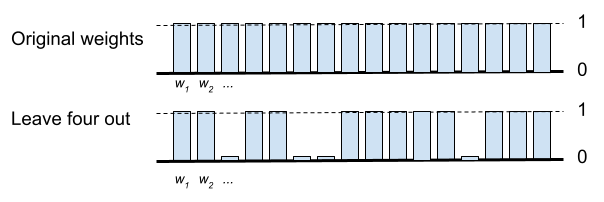
\includegraphics[width=0.9\linewidth]{static_figures/Weights2.png}}

\end{frame}


%%%%%%%%%%%%%%%%%%%%%%%%%%%%%%%%%%%%%%%%%%%%%%%%%%%%%%%%%%%%%%%%%%%%%%%%%%%%
%%%%%%%%%%%%%%%%%%%%%%%%%%%%%%%%%%%%%%%%%%%%%%%%%%%%%%%%%%%%%%%%%%%%%%%%%%%%
%%%%%%%%%%%%%%%%%%%%%%%%%%%%%%%%%%%%%%%%%%%%%%%%%%%%%%%%%%%%%%%%%%%%%%%%%%%%


\begin{frame}{Quantity of interest.}
%
\vspace{-2em}
\begin{align*}
%
\textrm{Z-estimator: }\quad
\thetahat(\w) :=
\theta \,\, \textrm{ such that } \,\,
\sumn \w_{n} G(\theta, \d_{n}) =  \zP .
%
\end{align*}
%
\pause

Fix some quantity of interest, $\phi(\w)$.  Examples:
%
\begin{align*}
    \phi(\w) =&{} \thetahat(\w)_p & \textrm{(A particular component of }\theta\textrm{)}\\
    \phi(\w) =&{} \thetahat(\w)_p + \frac{1.96}{\sqrt{N}} \hat\sigma(\thetahat(\w), \w)
        & \textrm{(The end of a confidence interval)}
\end{align*}
%
\pause
Let the \textbf{``signal''} be a ``large'' change $\Delta$ in $\thetafun$.
%
%\vspace{-0.5em}
%
\begin{columns}
%
\begin{column}{0.55\linewidth}
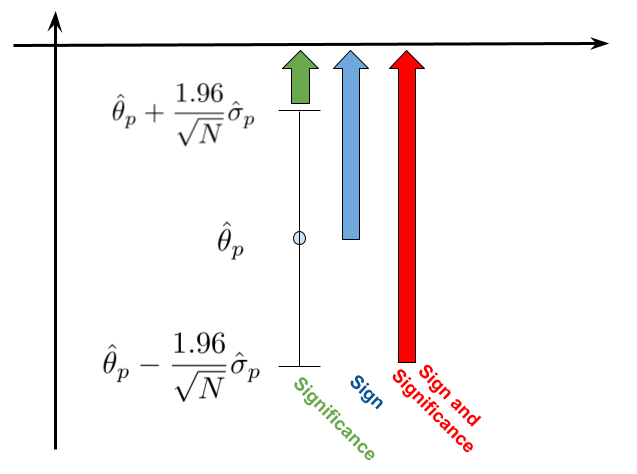
\includegraphics[width=0.95\linewidth]{static_figures/adversarial_robustness_example_phi_flipped.png}
\end{column}
%
\begin{column}{0.44\linewidth}
    \pause

    \begin{center}
        Are we robust to dropping $\lfloor \alpha N \rfloor$ datapoints?

        \textbf{$\Leftrightarrow$}

        Is there a $\w$, with no more than
        $\lfloor \alpha N \rfloor$ zeros, such that
        $\phi(\w) - \phi(\onevec) \ge \Delta$?
    \end{center}


\end{column}
\end{columns}

\end{frame}



%%%%%%%%%%%%%%%%%%%%%%%%%%%%%%%%%%%%%%%%%%%%%%%%%%%%%%%%%%%%%%%%%%%%%%%%%%%%
%%%%%%%%%%%%%%%%%%%%%%%%%%%%%%%%%%%%%%%%%%%%%%%%%%%%%%%%%%%%%%%%%%%%%%%%%%%%
%%%%%%%%%%%%%%%%%%%%%%%%%%%%%%%%%%%%%%%%%%%%%%%%%%%%%%%%%%%%%%%%%%%%%%%%%%%%


\begin{frame}{Taylor series approximation.}
%
Is there a $\w$, with
$\lfloor \alpha N \rfloor$ zeros, such that
$\thetafun(\w) - \thetafun(\onevec) \ge \Delta$?

\pause
\textbf{Hard!}
Evaluating $\thetafun(\w)$ exactly requires finding $\theta(\w)$ exactly.

\pause
\hrulefill

%\vspace{0.5em}
To simplify the search over $\w$, we form the Taylor series approximation:
%
\begin{align*}
	\thetafun(\w)
		&\approx
        \color{red}
        \thetafunlin(\w)
		:= \thetafun(\onevec) +
        \sumn (w_n - 1) \infl_n
        \color{black}
        , \textrm{ with } \infl_n :=
        \fracat{\partial \thetafun(\w)}{\partial w_n}{\w = \onevec}.
\end{align*}
%
\pause
The values $\infl_n$ are the ``influence function'', and can be \textbf{easily
and automatically} computed from $\thetahat(\onevec)$.
\citep{hampel1986robustbook}
%{\footnotesize \citep{hampel1986robustbook}}

The approximation is accurate (under mild conditions) for small $\alpha$.
\citep{giordano2019higherorder}

\pause
\hrulefill

Is there a $\w$, with
$\lfloor \alpha N \rfloor$ zeros, such that
$\color{red} \thetafunlin(\w) \color{black} - \thetafun(\onevec) \ge \Delta$?

\pause
\textbf{Easy!}
The most influential points for $\thetafunlin(\w)$ have the most negative
$\infl_n$.

\end{frame}


%%%%%%%%%%%%%%%%%%%%%%%%%%%%%%%%%%%%%%%%%%%%%%%%%%%%%%%%%%%%%%%%%%%%%%%%%%%%
%%%%%%%%%%%%%%%%%%%%%%%%%%%%%%%%%%%%%%%%%%%%%%%%%%%%%%%%%%%%%%%%%%%%%%%%%%%%
%%%%%%%%%%%%%%%%%%%%%%%%%%%%%%%%%%%%%%%%%%%%%%%%%%%%%%%%%%%%%%%%%%%%%%%%%%%%


\begin{frame}{Taylor series approximation.}

\textbf{Procedure:}

\begin{enumerate}
    \item<2-> Compute the ``original'' estimator, $\thetahat(\onevec)$ and
    $\thetafun(\onevec)$.
    \only<7->{\item[1.5] \textbf{Optional: } Compute $d\thetahat(\w) / d\w$.
        Then, for each interesting $\thetafun$:}
    \item<3-> Compute the sorted influence scores,
        $\infl_{(1)} \le \infl_{(2)} \le \ldots \le \infl_{(N)}$.
    \item<4-> Let $\w^*$ leave out the data corresponding to
    $\infl_{(1)},  \ldots , \infl_{(\lfloor \alpha N \rfloor)}$.
    %the $\lfloor \alpha N \rfloor$ most negative influence scores.
    \item<5-> Report non-robustness if
        $ \Delta \le \thetafunlin(\w^*) - \thetafun(\onevec)  =
            - \sum_{n=1}^{\lfloor \alpha N \rfloor} \infl_{(n)}$.
    \item<6-> \textbf{Optional: } compute $\thetahat(\w^*)$, and verify
    that $\Delta \le \thetafun(\w^*) - \thetafun(\onevec)$.
\end{enumerate}

\onslide<8->{
We have an \texttt{R} package, \texttt{rgiordan/zaminfluence},
    for OLS and IV.}

% \onslide<8->{
% \textbf{The above procedure can be automated using:}
% }


% \begin{itemize}
%     \item<8-> Code to compute $G(\theta, \d_n)$ and $\thetafun$,
%     \item<9-> The ``base solution'' $\thetahat(\onevec)$, and
%     \item<10-> Automatic differentiation. \citep{baydin2017automatic}
%     \item<11-> E.g., our \texttt{R} package, \texttt{rgiordan/zaminfluence}
%         for OLS and IV
% \end{itemize}


\end{frame}
